\chapter{Schlechtes Wetter}

\shorthandoff{"}
\dictum[\citeNP{nordwind2012rennradnews}]{"Direkt nach den Aufstehen aus dem Fenster geguckt und es war am Regnen und sehr Windig,
20min später losgefahren und siehe da der Regen hatte auf gehört und ich hatte den kompleten Weg zur Arbeit Rückenwind wie doof."}
\shorthandon{"}

\section{Kognitive Umstrukturierung}

Wenn man sich entscheidet, mit dem Rennrad zu pendeln gehört eine positive Grundhaltung zu \emph{jedem} Wetter dazu.
Es ist durchaus so, dass ich bei mildem, sonnigen Wetter (nicht zu heiss, nicht zu kalt) am liebsten fahre.
Nun ist das halt nicht immer der Fall. Die Schweiz hat gleichmässig etwa 12 bis 14 Regentage pro Monat.
D.h. dass im Schnitt es so an jedem dritten Tag mit Regen zu rechnen ist.
Wenn man Glück hat, sitzt man nicht gerade im Sattel, wenn dieses Nass vom Himmel kommt, sondern vorher oder nachher.
Trotzdem ist mit Nasswerden auch bei optimaler Planung und Studium des Wetterbrichtes immer zu rechnen.

Ein weiterer Trick ist, sich selbst kognitiv neu zu strukturieren (sprich: die Sache positiv zu sehen).
Zum Beispiel sich bewusst zu machen, dass die relativ kurze Distanz zur Arbeit nicht ausreicht, 
um wirklich auszukühlen oder wie Bradley Wiggins meint: <<It's not really long enough to get super-cold>> \cite{bbc2015wigginswinter}.

Für weitere Beispiele für die persönliche kognitive Umstrukturierung siehe Tabelle \ref{tab:kognitiveumstrukturierung}).

\begin{table}
        \centering
        \begin{tabular}{l}
                \toprule
        <<Nach 5 Minuten im Sattel spüre ich das Wetter nicht mehr.>>\\
        <<Genau jetzt hole ich mir den Trainingsvorteil gegenüber Schönwetterfahrern.>>\\
        <<Jetzt verbessere ich meine Fahrtechnik in Nässe und Kälte.>>\\
        <<Ich hole mir jetzt Rennhärte!>>\\
        <<Bei schönem Wetter fahren kann jeder.>>\\
        <<Nichts ist schöner, als nach einer solchen Fahrt unter die warme Dusche zu stehen.>>\\
        <<If you are out riding in bad weather, it means you are a badass. Period. \cite[Rule \#9]{velominati2014rules}\\
                \bottomrule
        \end{tabular}
        \caption{Kognitive Umstrukturierung: wichtig ist dabei sich einen für sich stimmige Grundüberzeugung zu finden.
        Diese muss dann möglichst oft ins Bewusstsein geholt werden, um verankert zu werden.}
        \label{tab:kognitiveumstrukturierung}
\end{table}

\section{Kälte}

\textbf{Luftdruck der Reifen reduzieren:}
\section{Regen}
\label{sec:regen}

Regen heisst in unseren Breitengraden: es ist Kalt \emph{und} Nass.
Das Thema Kälte wurde soeben angeschaut, hier kommt noch der Teil mit dem Nass.

Folgende Hinweise von \cite{Glass2014cyclingrain,Hurford2014rainyride,Prinz2014rain,Lovell2015tipswetweather,gcn2013rain,gcn2015rain}

Zur Motivation bei Fahrt im Regen \cite{Magnuson2013rain}

\subsection{Massnahmen am Rad}

\textbf{Schutzbleche montieren:}
<<Schutzbleche sind unästhetisch und gehören nicht ans Rennvelo.>>
Die, die so denken, fahren nicht oft bei Regen.
Nichts kann einem die Freude am Fahren schneller vermiesen als von unten mit dem ganzen Strassenschmutz bespritzt zu werden.
Zudem irrigiert der dauernd benässte Hintern. Ein nicht zu vernachlässigendes Sicherheitsrisiko.
An das Pendler-Rad gehören Schutzbleche.
Gepfiffen auf die Ästhetik -- oft ist ja sowieso dunkel.
Es geht ja auch um dem Trainingseffekt -- da stören die wenigen Gramm, die entsprechende Schutzbleche wiegen kaum.

\textbf{Breitere Reifen montieren:} 
Insbesondere bei Scheibenbremsen besteht die Möglichkeit, breitere Reifen zu montieren.
Das erhöht die Kontaktfläche Gummi--Strasse.

\textbf{Licht montieren:}
Ich spreche hier nicht von den kleinen Designerlämpchen, die man im Fahrradzubehör für die Rennradfraktion bekommt.
Ich spreche von LICHT!
Ich spreche Super-Mega-Watt-Funzeln, die durchaus geeignet sind, mit ihrem Lichtkegel fortlaufend die Strasse vor einem zu trocknen.
Erhältlich nur gegen Waffenschein im MTB-Zubehör.
Alles anderes ist Etepetete-Klinkerlitzen-Spielzeugkram.

\begin{figure}[<+htpb+>]
  \centering
  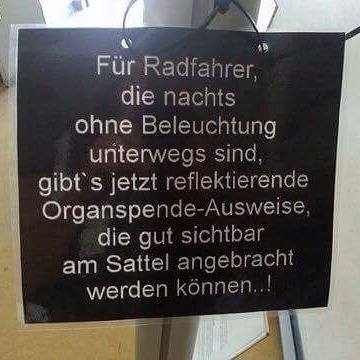
\includegraphics[width=0.5\textwidth]{figures/ohne-beleuchtung.jpg}
  \caption{Aus einem Facebook-Post \protect\cite{officepony2016organspendeausweis}},
  \label{fig:ohne-beleuchtung}
\end{figure}


\subsection{Kleidung/Ausrüstung}

\textbf{Brille:}
Ob jemand eine Brille bei Regen trägt, hängt meines Erachtens von der Situation ab.
Je nach Licht, Verkehr, Regenstärke finde ich eine Brille hilfreich oder störend.
Oft fahre ich dann ohne Brille.
Allerdings benutze ich Schutzbleche.
Ohne, dient eine Brille auch als Schutz von Spritzer von Regen und hochgeschleudertem Strasendreck dienen sie auch der Sicherheit.
Ausgerüstet mit gelben oder orangen Gläsern, erhöhen sie den Kontrast.

\textbf{Radfahrerkappe unter Helm:}
Neben dem Profi-mässigen Aussehen dient der Schirm noch etwas dazu, die Augen zu schützen.
Allenfalls entschliesst man sich sogar für den Kauf eines MTB-Helmes mit Schirm.

\textbf{Überzieh-Handschuhe:}
Als meine Wetter-Schwachstelle würde ich die Finger bezeichnen.
So ungerne ich an die Finger friere, so ungern habe ich es dort zu warm.
Diesbezüglich habe ich ein kleines Sortiment an unterschiedlich gefütterten Handschuhen.
Neben den wasserfesten Winterhandschuhe (gegen Nässe und Kälte) gibt es im Handel auch dünne Sommer-Regen-Überziehhandschuhe
(z.B. Roeckl Malvas).
Wem auch eine unkonventionellen Lösung genehm ist und damit leben kann, auf dem Rennvelo wie ein Chirurg auszusehen,
kann sich im Falle eines Wolkenbruches auch ein Paar Latex-Handschuhe überziehen.
Ich persönlich werde dann halt lieber nass.

\textbf{Regenüberschuhe/wasserdichte Socken:}
Die Regenüberschuhe sollten so beschaffen sein, dass sie einfach an- und ausgezogen werden.
Ich führe \emph{immer} ein Paar im Rucksack.
Wenn die Radschuhe erst einmal so richtig durchnässt sind,
kann es Tage gehen, bis sie wieder trocken sind.

\textbf{Regentaugliche Kleidung:}
Grundsätzlich sollte gerade bei Regen auf leuchtende, reflektierende Kleidung getragen werden.
Je bunter desto besser?
Mit der üblichen Funktionskleidung wirkt man bei der Normalbevölkerung sowieso etwas seltsam \cite{Rasche2016albern}.
Aber eigentlich ist egal, was andere denken, wenn es der eigenen Sicherheit und Komfort dient.
Bei Nässe kann man sich für grundsätzlich für eine \textsl{hard shell} oder \textsl{soft shell} entscheiden.
Während eine hard shell mehr wasserdicht ist aber weniger Ventilation (Schweiss) zulässt und eher für lange Ausfahrten geeignet ist \cite{gcn2015rain},
ist bei den eher kurzen, harten Fahrten zum Pendlen eine soft shell geeigent (wohl weniger wasserdicht, lässt mehr ventilation zu, weniger geflatter).

\textbf{Rucksack mit Regenüberzug:}
Ist sicher tivial, scheint mir aber aus folgenden Punkten im Bezug aufs Pendeln erwähnenswert.
Mehr als früher montiere ich den Regenüberzug schon im Voraus.
Es nervt, bei der Fahrt wegen einsetzendem Regen anzuhalten und ihn nachträglich zu montieren.
Gerne lässt man es dann bleiben und ärgert sich dann über durchnässtes Arbeitsmaterial.
Zudem ist der Regenüberzug oft durch Farbgebung und Reflexionsstreifen noch etwas auffälliger als der Rucksack selbst,
was die Sicherheit erhöht.

\textbf{Handy in Gefrierbeutel:}
Wenn nicht schon im Rucksack lohnt sich für z.B. für das Handy ein Gefrierbeutel mit Clipverschluss.
Das mache ich auch bei trockenem Wetter zum Schutz vor Schweiss.

\textbf{Sitzcreme auftragen:}
Global Cycling Network empfielt noch speziell bei Regen das Auftragen von Sitzcreme \cite{gcn2013rain,gcn2015rain}.
Die Begründung des Schutzes der feuchten Haut leuchtet ein, das ist aber kaum nur ein Problem bei Regen,
die Stelle wird auch bei trockenen Ausfahrten nass durch den Schweiss.
Generall wird Sitzcreme (günstige Alternative ist Melkfett) bei langen Ausfahrten als Schutz vor dem Wundscheuern empfohlen.
Ob sich persönlich der Extraaufwand für die vergleichsweise kurze Strecke lohnt, muss jeder für sich ausprobieren.

\subsection{Verhalten}

\textbf{Löcher und Pfützen meiden:}
Man soll dem kindlichen Impuls widerstehen, durch Pfützen zu fahren.
Auch unter einer harmlosen kleinen Wasserlache kann ein tieferes Loch oder eine Glasscherbe lauern.

\textbf{Vorsicht bei Strassensignalisationen, Gulli-Deckel, Tram-Schienen:}
Man soll sich das eigentlich schon bei trockenem Wetter angewöhnen.
Strassenbemalungen und Gullideckel sind tabu.
Insbesondere die Kombination Gummi und nasses Metall ist wie Schmierseife.

\textbf{Geschwindigkeit anpassen:}
Bei Nässe haften die Räder nur noch halb so gut wie im Trockenen (Tabelle \ref{tab:haftreibung}).
Neben der schlechteren Strassenhaftung ist die eigene Sicht stark eingeschränkt.
Zudem funktionieren die (Felgen-)Bremsen wie gewohnt.
Die Räder blockieren viel schneller, was den Bremseffekt weiter schwächt.

\begin{table}
  \centering
  \begin{tabular}{ll}
    \toprule
    Strassenzustand & Haftreibungungszahl \\
    \midrule
    trocken         & 0.7 -- 0.1 \\
    nass            & 0.4 -- 0.6 \\
    nasses Laub, Schnee & 0.2 -- 0.3 \\
    bei Eis         & 0.1 \\
    \bottomrule
  \end{tabular}
  \caption{Haftreibungszahl von Luftreifen bei verschiedenen Strassenzuständen \protect\cite{Strommer2016haftreibung}}
  \label{tab:haftreibung}
\end{table}


\textbf{Bremsen trocken bremsen:}
Gerade vor Kreuzungen oder geplanten Stopps kann man schon gefühlvoll etwas vorbremsen.
Man vermeidet so die Schrecksekunde, wenn die Felgenbremsen im Nassen nicht reagieren.

\textbf{Gefühlvoll in die Kurve:}
Weniger Haftung, schlechte Sicht.
Zwei Gründe, wieso gerade in der Kurve vorsichtig gefahren werden muss.

\textbf{Vorhersehbar fahren:}
Für andere Verkehrsteilnehmer mitdenken.
Gerade bei Regen ist die Sicht auch für andere Verkehrsteilnehmer eingeschränkt.
Umsomehr soll man alles vermeiden, was gerade Autofahrer irritiert (Slalom, Vortritt missachten).
Hypervorsicht und pingeliges Einhalten von Verkehrsregeln ist hier angesagt.

\textbf{Regenfahrt geniessen:}
Das scheint mir fast der wichtigste Punkt.
Keine Panik vor Regen!
Wenn man sich dem Wetter hingibt und in sich hineinfühlt merkt man plötzlich: es ist gar nicht schlimm.
Sondern es macht ja Spass!
Das Licht ist anderst, die Geräusche sind anderst. Man sieht die Tropfen vom Rad springen.
Man fährt anderst, weicht den Pfützen aus, vermeidet Gullis.
Regen auf dem Gesicht wäscht den Schweiss weg.
Man spührt, dass gegen die Hitze der Anstrengung die Kühle des Regens einem gut tut.

